\documentclass[tikz,border=1.35mm]{standalone}

\definecolor{fvmadaptedge}{HTML}{8A7E7E}
\usetikzlibrary{arrows.meta}

\definecolor{splitred}{HTML}{AF2525}

% Irregular six-sided face before and after isotropic face splitting.
% Coordinates are in millimeters; y=-1mm keeps the SVG-style origin at top left.
\begin{document}
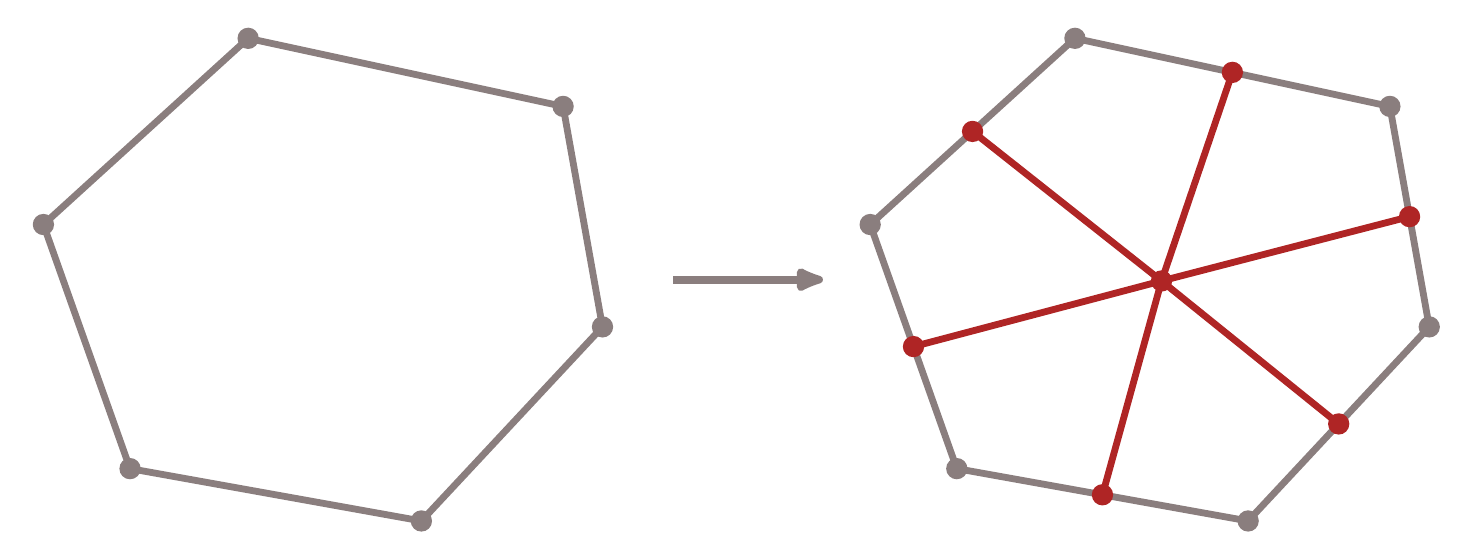
\begin{tikzpicture}[
  x=1mm,
  y=-1mm,
  line join=round,
  edge/.style={draw=fvmadaptedge,line width=0.865mm},
  splitline/.style={draw=splitred,line width=0.865mm},
  arrow/.style={draw=fvmadaptedge,line width=1.05mm,-{Latex[round,length=4.8mm,width=3.6mm]}}
]
  % Match the artwork frame before the standalone border is applied.
  \useasboundingbox (0,0) rectangle (181.000,64.000);

  % Left panel: original unsplit irregular face.
  \coordinate (a0) at (28.000,1.353);
  \coordinate (a1) at (68.000,10.000);
  \coordinate (a2) at (73.000,38.000);
  \coordinate (a3) at (50.000,62.647);
  \coordinate (a4) at (13.000,56.000);
  \coordinate (a5) at (2.000,25.000);

  % Right panel: original vertices, edge midpoints, and face center.
  \coordinate (b0) at (133.000,1.353);
  \coordinate (b1) at (173.000,10.000);
  \coordinate (b2) at (178.000,38.000);
  \coordinate (b3) at (155.000,62.647);
  \coordinate (b4) at (118.000,56.000);
  \coordinate (b5) at (107.000,25.000);
  \coordinate (m01) at (153.000,5.677);
  \coordinate (m12) at (175.500,24.000);
  \coordinate (m23) at (166.500,50.324);
  \coordinate (m34) at (136.500,59.324);
  \coordinate (m45) at (112.500,40.500);
  \coordinate (m50) at (120.000,13.177);
  \coordinate (center) at (144.000,32.167);

  % Draw the old face and the split face topology.
  \draw[edge] (a0) -- (a1) -- (a2) -- (a3) -- (a4) -- (a5) -- cycle;
  \draw[edge] (b0) -- (m01) -- (b1) -- (m12) -- (b2) -- (m23)
    -- (b3) -- (m34) -- (b4) -- (m45) -- (b5) -- (m50) -- cycle;
  \foreach \p in {m01,m12,m23,m34,m45,m50} {
    \draw[splitline] (center) -- (\p);
  }

  % Transformation arrow between the before/after panels.
  \draw[arrow] (82.000,32.000) -- (101.000,32.000);

  % Original vertices are #8a7e7e.
  \foreach \p in {a0,a1,a2,a3,a4,a5,b0,b1,b2,b3,b4,b5} {
    \fill[fvmadaptedge] (\p) circle[radius=1.353mm];
  }

  % Split-created edge and face nodes are red.
  \foreach \p in {m01,m12,m23,m34,m45,m50,center} {
    \fill[splitred] (\p) circle[radius=1.353mm];
  }
\end{tikzpicture}
\end{document}
